\documentclass{article}
\usepackage{tikz}
\usetikzlibrary{shapes}
\begin{document}
	The vector graphic will now be introduced:
	\begin{figure}[h!]
		\centering
		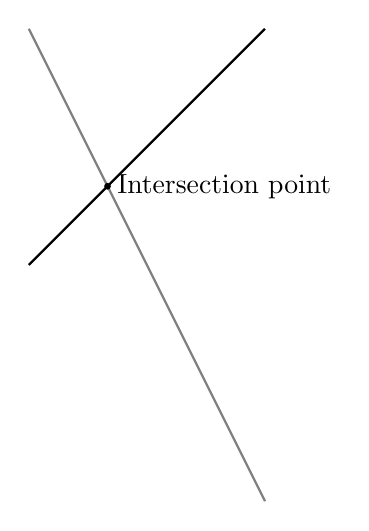
\begin{tikzpicture}
			\draw[gray, thick] (-1,2) -- (2,-4);
			\draw[black, thick] (-1,-1) -- (2,2);
			\filldraw[black] (0,0) circle (1pt) node[anchor=west]{Intersection point};
%			\node[regular polygon, regular polygon sides=3, draw=black, fill=black, minimum size=3pt, inner sep=0pt] at (0,0) {};
%			\node[anchor=west] at (0,0) {Intersection point};
		\end{tikzpicture}
	\end{figure}
\end{document}